\chapter{Utilisation du casque EPOC et d'OpenViBE}
\label{Chapitre : Utilisation du casque EPOC et d'OpenViBE}
\thispagestyle{fancy}

\section{OpenViBE}
\label{Section : 5.OpenViBE}

\subsection{Généralités sur le fonctionnement d'OpenViBE}
\label{Subsection : 5.Généralités sur le fonctionnement d'OpenViBE}
OpenViBE est une plateforme logicielle dédiée à la conception et à l'utilisation d'interfaces cerveau-ordinateur en temps réel. Celle-ci est éditée par l'Institut National de Recherche en Informatique et en Automatique (INRIA) de Rennes en France. Le logiciel gère à la fois l'acquisition, le traitement et l'analyse des signaux.

OpenViBE fonctionne sous forme de scénarios, correspondant à un ensemble de blocs fonctionnels. La suite OpenViBE est composée de deux logiciels : 
\smallbreak
\begin{itemize}
	\item \textbf{OpenViBE designer}. Il s'agit d'un éditeur de scénario permettant de  créer et modifier les schémas blocs grâce à une interface graphique. Il suffit alors de placer les différents blocs désirés, de les configurer (en cliquant dessus), et de les relier pour former une chaine de traitement (procédure).
	\smallbreak
	\item \textbf{OpenViBE acquisition server.} Permet d'acquérir des données EEG brutes à partir d'un dispositif EEG. Il est par exemple possible de connecter différents types de casques comme le casque EPOC d'Emotiv.
	\smallbreak
\end{itemize}

Il est possible d'envoyer des données d'OpenVIBE vers une application externe via une connexion VRPN (Virtual Reality Peripheral Network).

\subsection{Installation d'OpenViBE}
\label{Subsection : 5.Installation d'OpenViBE}
 Le logiciel fonctionne sous les systèmes d'exploitations Windows (Windows XP ou ultérieur, la stabilité du logiciel sous Windows 8 n'ayant pas été vérifiée par l'éditeur) et Linux (Ubuntu, Fedora). La liste détaillée des architectures compatibles avec OpenViBE est disponible à l'adresse suivante : http://openvibe.inria.fr/supported-architectures/.
Il est possible de télécharger l'installeur OpenViBE à l'adresse suivante : http://openvibe.inria.fr/downloads/. Une fois celui-ci téléchargé, il suffit de l'ouvrir et de suivre les indications affichées à l'écran.

\subsection{Utilisation d'OpenViBE designer}
\label{Subsection :5.Utilisation d'OpenViBE designer}

\subsubsection{Description de l'interface de contrôle de la simulation}
\label{Subsubsection : 5.Description de l'interface de contrôle de la simulation}
La partie supérieure de l'interface graphique permet de contrôler la simulation, i.e. le déroulement du scénario. Ainsi, il est possible de lancer un scénario en appuyant sur le bouton "lecture", de le stopper en appuyant sur le bouton "stop", d'en accélérer le déroulement en appuyant sur le bouton "avance rapide", etc. Il est également possible de lancer plusieurs scénarios en même temps (Figure : \ref{fig:interface_simu_ov}). 

\begin{figure}[h]
	\centering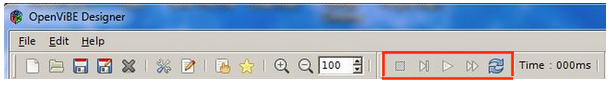
\includegraphics[height=2cm]{images/interface_simu_ov.png}
	\caption{Interface de contrôle de la simulation sous OpenViBE.}
	\label{fig:interface_simu_ov}
\end{figure}

\subsubsection{Description de l'interface du répertoire des blocs fonctionnels}
\label{Subsubsection : 5.Description de l'interface du répertoire de blocs fonctionnels}
La partie située à droite de l'interface graphique de l'éditeur permet de rechercher les blocs désirés afin de construire un scénario. Ceux-ci sont triés en différentes catégories. un simple glisser-déposer permet de placer un bloc dans l'espace de travail (Figure : \ref{fig:interface_bloc_ov}).

\begin{figure}[h]
	\centering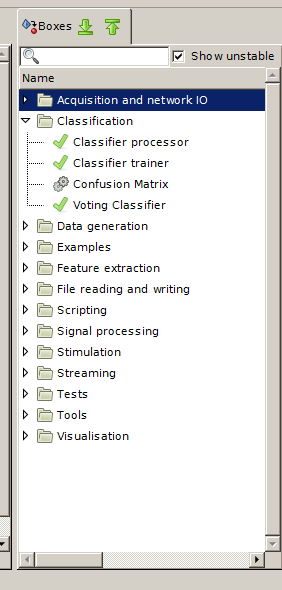
\includegraphics[height=7cm]{images/interface_bloc_ov.png}
	\caption{Interface du répertoire des blocs OpenViBE.}
	\label{fig:interface_bloc_ov}
\end{figure}

\subsubsection{Description de l'espace de travail}
\label{Subsubsection : 5.Description de l'espace de travail}
La partie centrale de l'interface graphique correspond à l'espace de travail d'OpenViBE. C'est ici où l'on construit les différents scénarios de l'interface cerveau-ordinateur, via des blocs fonctionnels. Chaque bloc peut être relié à un autre en maintenant la souris sur la sortie d'un bloc, vers l'entrée d'un autre bloc. On peut seulement connecter une entrée à une sortie du même type (e.g. une entrée de type "signal" vers une sortie de type "signal") (Figure : \ref{fig:interface_travail_ov}).

\begin{figure}[h]
	\centering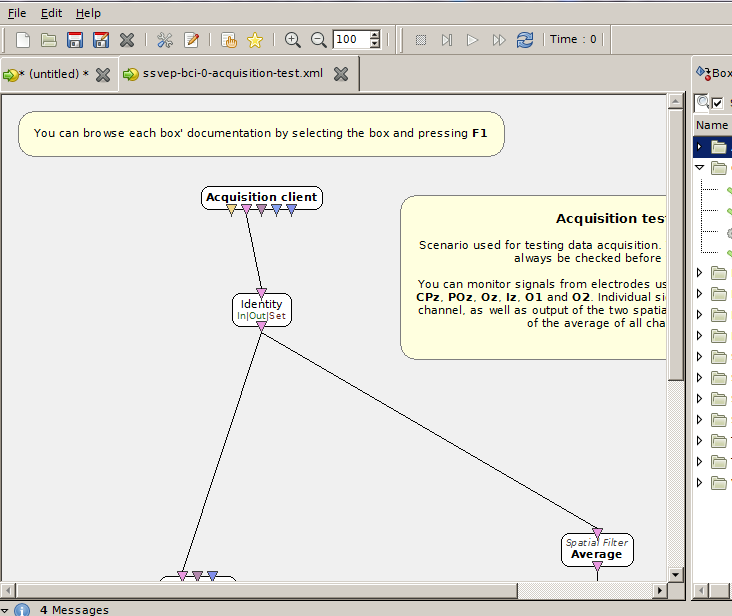
\includegraphics[height=8cm]{images/interface_travail_ov.png}
	\caption{Espace de travail d'OpenViBE.}
	\label{fig:interface_travail_ov}
\end{figure}

\subsection{Description des blocs utilisés}
\label{Subsection : 5.Description des blocs utilisés}
Voici la liste des différents blocs utilisés dans le cadre de notre projet :

\subsubsection{Acquisition et Réseau}
\label{Subsubsection : 5.Acquisition et Réseau}
\begin{itemize}
	\smallbreak
	\item \textbf{Acquisition Client.} Ouvre une interface de connexion pour lire les information envoyées par le serveur d'acquisition (i.e. les données du casque en temps réel). Il faut pour cela indiquer le port utilisé par le serveur (1024 par défaut).
	\smallbreak
	\item \textbf{Analog VRPN Server.} Permet d'envoyer des données à une application client via le protocole VRPN.
\end{itemize}
\subsubsection{Traitement de signal}
\label{Subsubsection : 5.Traitement de signal}
\begin{itemize}
	\smallbreak
	\item \textbf{Temporal Filter}. Réalise le filtrage temporel d'un signal. Il est possible de choisir la méthode de filtrage (passe-bas, passe-bande ou passe-haut), le type (Butterworth, Chebychev) et l'ordre de filtre.
	\smallbreak
	\item \textbf{Spatial Filter}. Permet de réaliser un filtrage spatiale statique, i.e. en paramétrant le poids attribué à chaque canal d'entrée manuellement. (filtrage bipolaire, Laplacien, etc.)
	\smallbreak
	\item \textbf{FastICA.} Permet de réaliser un filtrage spatial via l'algorithme ICA (\ref{Subsecton : 4.ICA}). Attention, le bloc est cependant considéré comme non stable par l'INRIA.
	\smallbreak
	\item \textbf{CSP Spatial Filter Trainer.} Permet réaliser un filtrage spatial via l'algorithme CSP (\ref{Subsubsecton : 4.CSP}).
	\smallbreak
	\item  \textbf{Time Based Epoching.} Permet de découper un signal en plusieurs morceaux ayant une durée et un intervalle spécifié.
	\smallbreak
	\item \textbf{Simple DSP.} Permet de réaliser des algorithmes mathématiques simples.
	\smallbreak
	\item \textbf{Signal Average.} Permet de calculer la moyenne d'un signal.
	\smallbreak
	\item \textbf{Spectral Analysis (FFT).} Réalise l'analyse spectrale de signaux en utilisant la FFT (Fast Fourier Transform).
	\smallbreak
	\item \textbf{ Spectrum Average.} Calcule la moyenne de toutes les puissances de bande de fréquence pour un spectre donné.
\end{itemize}
\subsubsection{Classification}
\label{Subsubsection : 5.Classification}
\begin{itemize}
	\smallbreak
	\item \textbf{Classifier Trainer.} Permet de réaliser des algorithmes de classification. Ce bloc effectue plus particulièrement l'entrainement du classificateur. Les différents algorithmes proposés sont la LDA et la SVM.
	\smallbreak
	\item \textbf{Classifier Processor.} Permet de réaliser la classification de vecteurs  caractéristiques entrants, en utilisant un classificateur entrainé précédemment.
	
\end{itemize}
\subsubsection{Lecture et écriture de fichiers}
\label{Subsubsection : 5.Lecture et écriture de fichiers}
\begin{itemize}
	\smallbreak
	\item \textbf{Generic Stream Writer.} Permet d'écrire des données dans un fichier binaire. Extension du fichier : .ov
	\smallbreak
	\item \textbf{Generic Stream Reader.} Permet de lire un fichier enregistré grâce à un bloc Generic File Writer.
	\item \textbf{CSV File Reader.} Ce bloc permet de lire des données (signaux par exemple) issues d'un fichier CSV (Comma-Separated Values). Le format  CSV est ouvert et représente les données sous la forme de valeurs séparées par des virgules (format Européen), des points-virgules (format Américain) ou des tabulations. Ce bloc peut-être utilisé pour réaliser l'importation de données depuis Matlab ou Octave. 
	\smallbreak
	\item \textbf{CSV File Writer.} Ce bloc permet d'écrire des données issues d'OpenViBE dans un fichier CSV. Il peut par exemple être utilisé pour réaliser de l'exportation de données vers Matlab ou Octave.
\end{itemize}
\subsubsection{Simulation}
\label{Subsubsection : 5.Simulation}
\begin{itemize}
	\smallbreak
	\item\textbf{Player Controller.} Permet de contrôler l'arrêt et la mise en pause d'un scénario à l'aide des stimulations reçues. 
\end{itemize}
\subsubsection{Visualisation}
\label{Subsubsection : 5.Visualisation}
\begin{itemize}
	\smallbreak
	\item\textbf{Signal Display.} Permet d'afficher un signal en temps réel.
	\smallbreak
	\item\textbf{Power Spectrum Display.} Permet d'afficher l'amplitude d'un signal dans un ensemble de bandes de fréquences.
	\smallbreak
	\item \textbf{2D Topographic Map.} Permet d'afficher la topographie de l'activité cérébrale en 2 dimensions.
	\smallbreak
	\item \textbf{3D Topographic Map.} Permet d'afficher la topographie de l'activité cérébrale en 3 dimensions.
	\smallbreak
	\item\textbf{Graz Visualisation.} Permet d'afficher la consigne et le résultat en temps réel.
\end{itemize}
\subsubsection{Autres}
\label{Subsubsection : 5.Autres}
\begin{itemize}
	\smallbreak
	\item \textbf{Feature aggregator.} Permet de rassembler les différentes entrées du bloc vers un vecteur caractéristique.
	\smallbreak
	\item\textbf{Identity }. Duplique l'entrée de ce bloc vers sa sortie.
\end{itemize}


\subsection {Utilisation du serveur d'acquisition d'OpenViBE}
\label{Subsection : 5.Utilisation de OpenViBE acquisition Server}
On s'appuie ici sur l'utilisation d'OpenViBE acquision server afin d'acquérir les données EEG brutes à partir du casque EPOC (composé, pour rappel, de 14 canaux EEG). Afin d'accéder à ces données, il est nécessaire d'être en possession du SDK de ce casque (édition de recherche). De plus, il est nécessaire d'utiliser le système d'exploitation Windows afin d'assurer la compatibilité d'OpenVIBE avec le casque EPOC.

Au lancement du serveur d'acquisition d'OpenViBE, la fenêtre de configuration apparait (Figure \ref{fig:acquisition}, fenêtre de gauche).
\smallbreak
\begin{itemize}
	\item \textbf{Driver}. Indiquer le pilote correspondant au casque utilisé via le menu déroulant. Il s'agit dans notre cas du casque EPOC d'Emotiv.
	\smallbreak
	\item \textbf{Connection Port}. Permet de renseigner le port de connexion du casque. Laisser la valeur à 1024.
	\smallbreak
	\item \textbf{Sample count per sent block}. Permet de configurer la taille des paquets envoyés du casque vers OpenViBE. Laisser à 32.
	\smallbreak
\end{itemize} 

Appuyer sur le bouton "Driver properties" ouvre la fenêtre de configuration du casque (Figure \ref{fig:acquisition}, fenêtre de droite). Il faut alors renseigner les champs suivants :
\smallbreak
\begin{itemize}
	\item \textbf{Identifier}. Permet d'enregistrer les données de plusieurs utilisateurs. Laisser la valeur à 0.
	\smallbreak
	\item \textbf{Age}. Renseigner l'âge de l'utilisateur.
	\smallbreak
	\item \textbf{Gender}. Renseigner le sexe de l'utilisateur.
	\smallbreak
\end{itemize}


\begin{figure}[h]
	\centering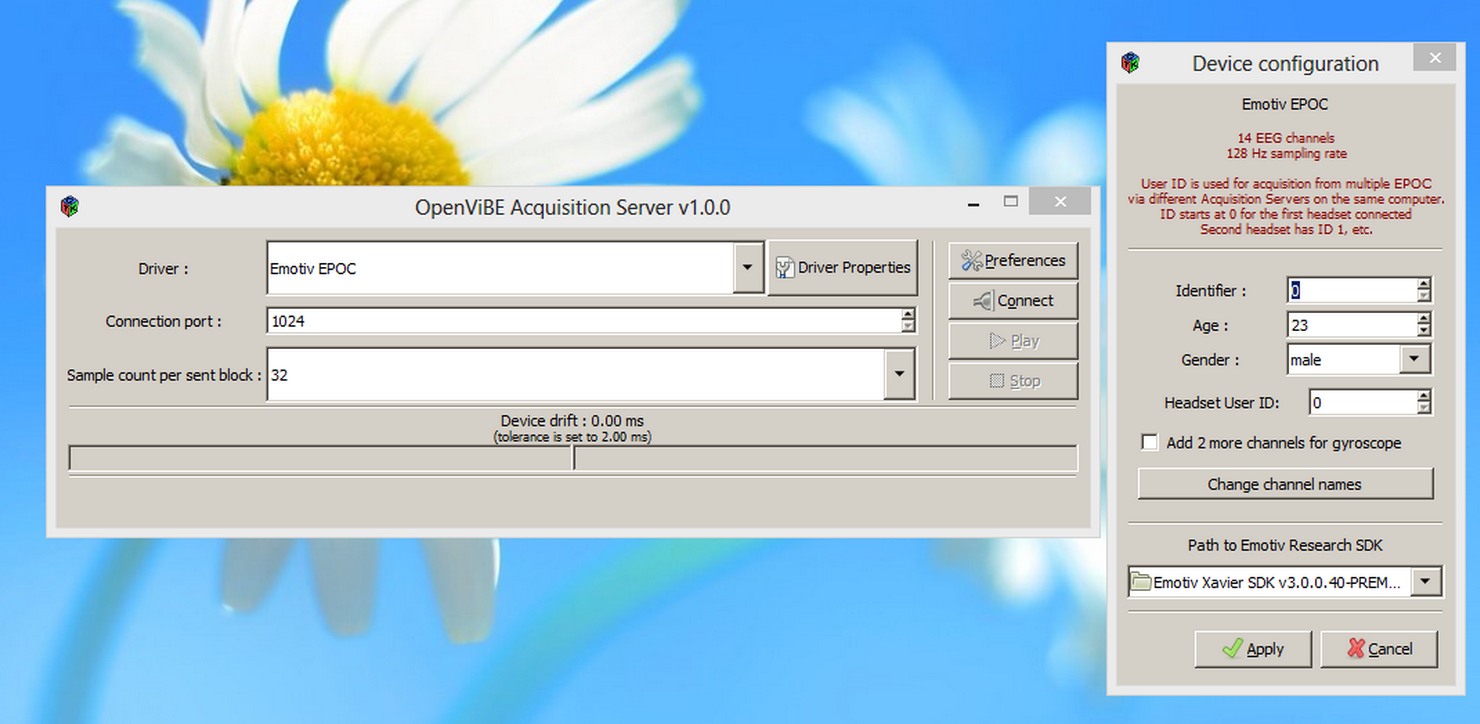
\includegraphics[height=6.5cm]{images/configOpenvibeEpoc.png}
	\caption{Lancement du serveur d'acquisition}
	\label{fig:acquisition}
\end{figure}

Ensuite, il ne reste plus qu'à appuyer sur "Connect" et sur "Play". La connexion entre le casque et OpenViBE s'effectue alors via le serveur d'acquisition. Le message "Connection succeded" informe l'utilisateur que la connexion avec le casque a été réalisée (Figure \ref{serveurUp}).

\begin{figure}[h]
	\centering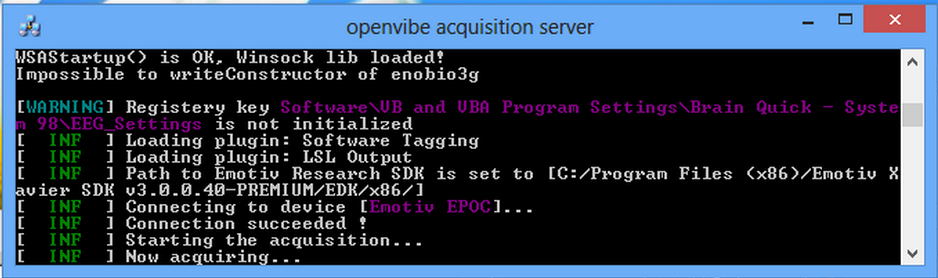
\includegraphics[height=3.5cm]{images/serveurUp.png}
	\caption{Serveur démarré}
	\label{serveurUp}
\end{figure}

\section {Utilisation du casque EPOC}
\label{Section : 5.Utilisation du casque EPOC}

\subsection{Généralités sur le fonctionnement du casque}
\label{Subsection : 5.Généralités sur le fonctionnement du casque}
Afin d'utiliser le casque EPOC d'Emotiv et d'acquérir les données EEG, il est nécessaire d'utiliser deux éléments :
\smallbreak
\begin{itemize}
	\item \textbf{Emotiv Xavier Control Panel Premium.} Il s'agit du panneau de configuration du casque EPOC. Il permet de le configurer et de le tester via une interface graphique.
	\smallbreak
	\item \textbf{ SDK Emotiv.} Il s'agit du kit de développement du casque. Dans le cadre de notre projet, il nous permettra d'utiliser le casque avec OpenViBE et d'acquérir les signaux EEG.
\end{itemize}
	
\subsection {Installation de Emotiv Xavier Control Panel Premium et du SDK.}
\label{Subsection : 5.Installation de Emotiv Xavier Control Panel Premier et du SDK}
Pour installer les deux utilitaires, il faut suivre la démarche suivante : 
\smallbreak
\begin{enumerate}
	\item Se connecter sur son compte Emotiv (https://emotiv.com/).
	\item Aller dans l'onglet "my downloads".
	\item Télécharger le SDK du casque.
	\item Une fois l'installeur téléchargé, l'ouvrir et suivre les instructions affichées à l'écran. Il vous sera demandé de fournir le code de la licence. Celui-ci est indiqué sur la page de téléchargement. L'installation de l'Emotiv Xavier Control Panel Premium s'effectuera lors de l'installation du SDK.
\end{enumerate}

\subsection {Préparation du casque}
\label{Subsection : 5.Préparation du casque}
Voici les étapes de préparation du casque : 
\smallbreak
\begin{enumerate}
	\item Bien humidifier chaque électrode avec la solution saline (jusqu’à saturation).
	\item Insérer ces électrodes sur le casque (il faut sentir un cran).
	\item Brancher la clé USB pour assurer la connexion sans fil avec le casque.
	\item Allumer le casque.
\end{enumerate}

\subsection {Conseils sur l'utilisation du casque}
\label{Subsection : 5.Conseils sur l'utilisation du casque}
\begin{itemize}
	\item Ré-hydrater les électrodes toutes les heures pour garantir un bon contact dermal et donc un signal optimal.
	\smallbreak
	\item S’assurer du bon fonctionnement du casque en vérifiant régulièrement la qualité du signal via le logiciel "Emotiv Xavier Control Panel Premium".
	\smallbreak
	\item Ranger les électrodes dans leur boite lorsque le casque n’est pas utilisé et s’assurer que le tampon soit humide (dans le cas contraire, l’humidifier avec la solution saline).
	\smallbreak
	\item Utiliser un tampon alcoolisé pour désinfecter les électrodes lorsque le casque n'est plus utilisé.
	\smallbreak
	\item Ne pas utiliser le casque lorsque sa batterie est en rechargement.
\end{itemize}

\subsection {Vérification de la qualité des signaux}
\label{Subsection : 5.Vérification de la qualité des signaux}
Afin d'exploiter de manière optimale les données provenant du casque, il est nécessaire de vérifier la qualité du signal à partir du panneau de configuration du casque. Lors de l'ouverture logiciel, et après connexion, le menu principal apparait. Sur l'interface, les différentes électrodes sont représentées par des points. Un points vert représente un signal de bonne qualité, un point orange de moyenne qualité et un point rouge ou noir correspond à un signal de mauvaise qualité (Figure \ref{qualiteSignal}).
	
\begin{figure}[h]
	\centering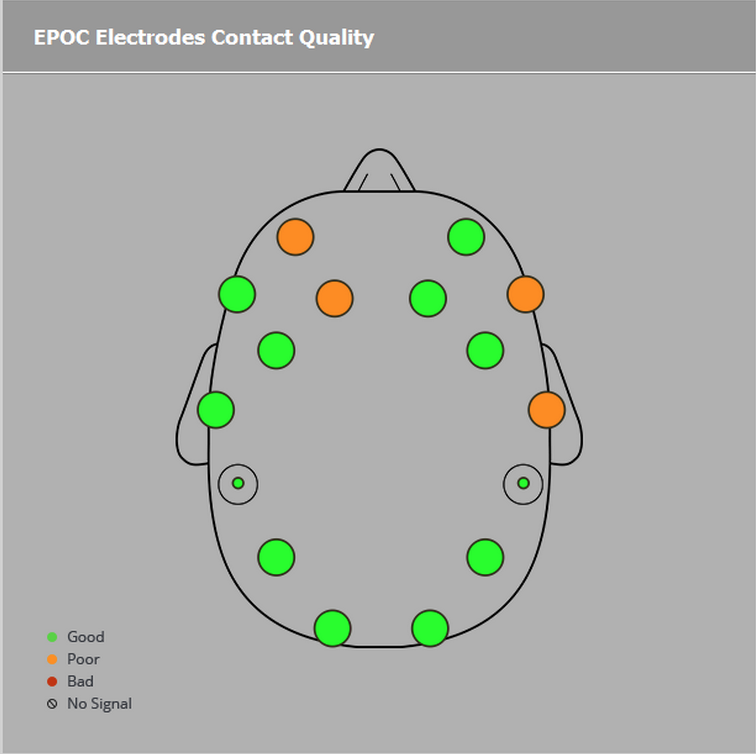
\includegraphics[height=6.5cm]{images/emotivQuality.png}
	\caption{Qualité du signal provenant des électrodes}
	\label{qualiteSignal}
\end{figure}
	